\chapter{GroundBIRD実験}
\label{chapter2}

CMB観測実験には地上から観測する実験と衛星を用いて宇宙から観測する実験に分けられる。ここでは私が参加しているGroundBIRD実験(図\ref{GB_overview})について実験の概要と現在の観測状況について説明する。

\begin{figure}[htbp]
  \centering
  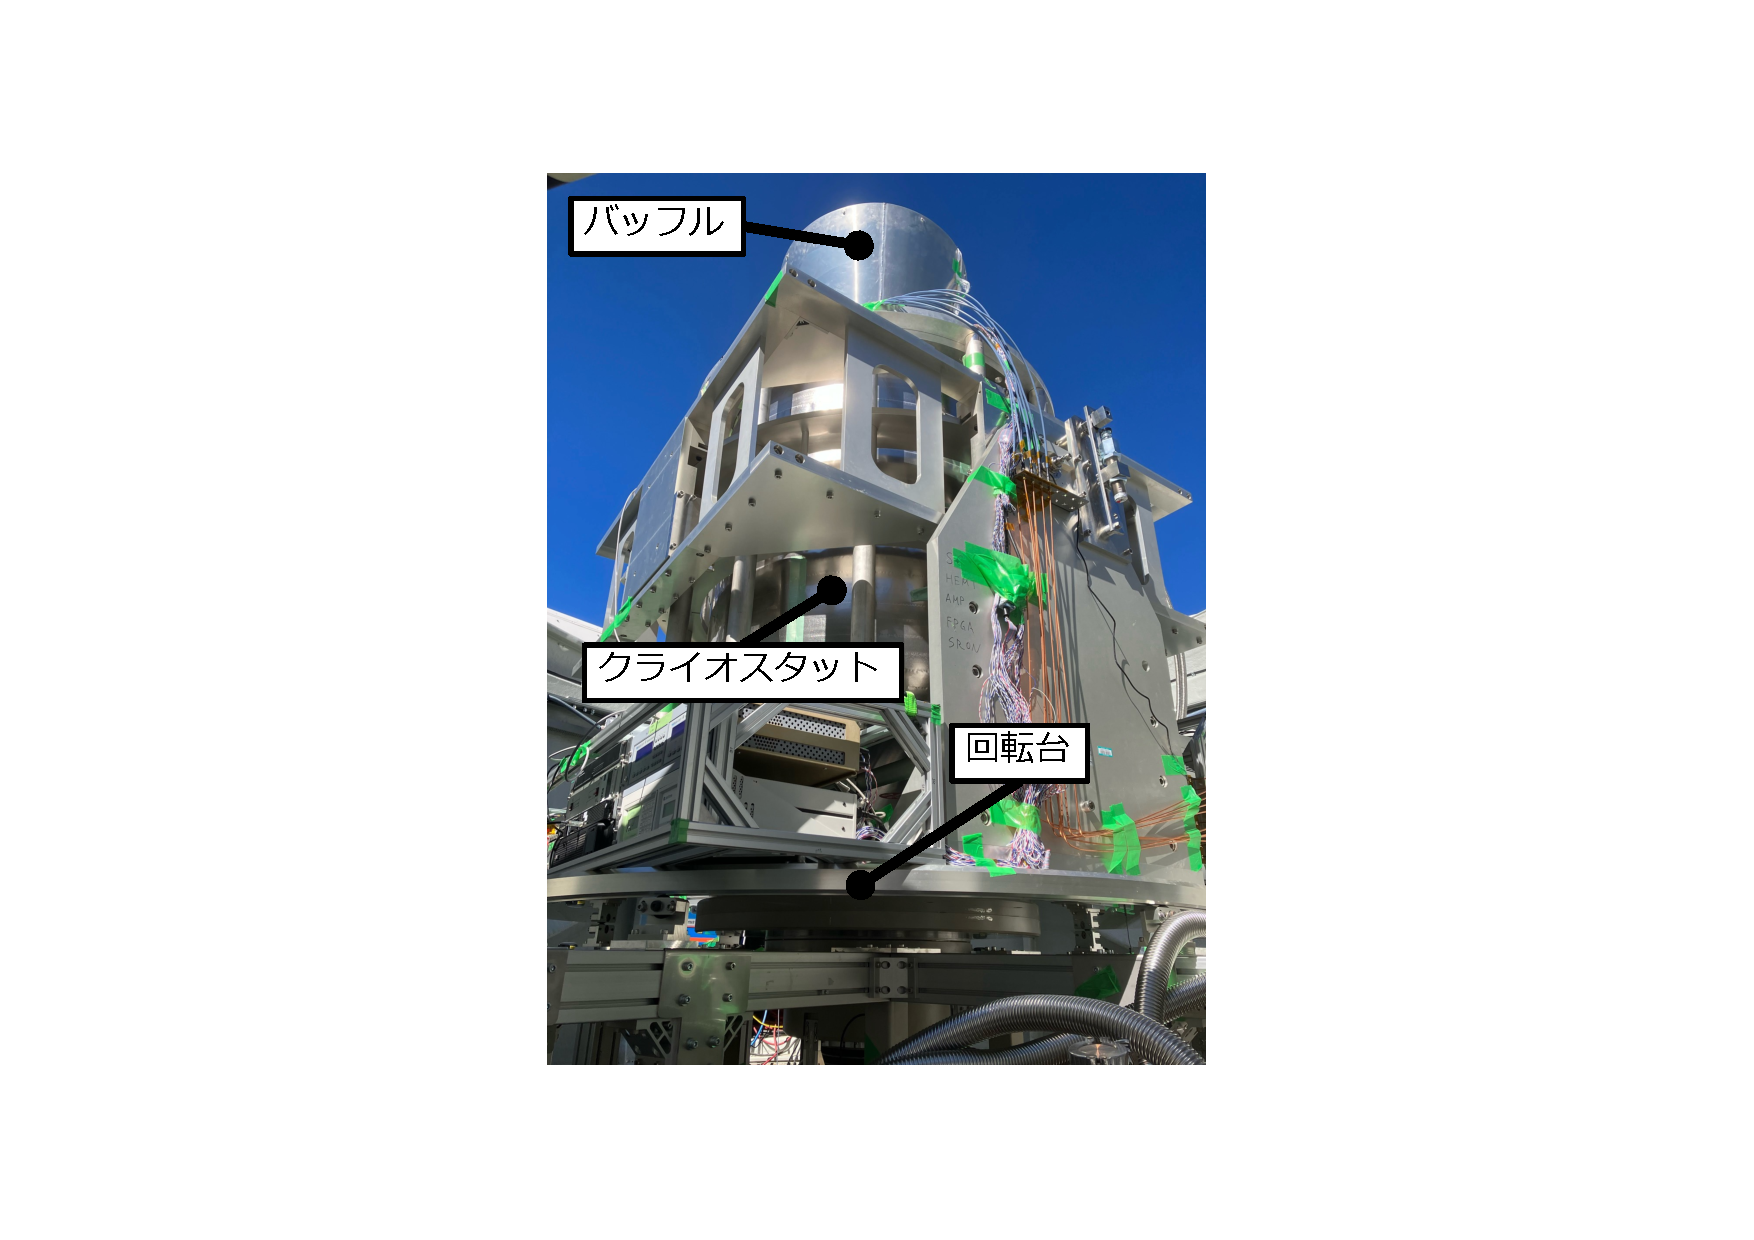
\includegraphics[width=0.5\columnwidth]{3_GB/figs/GB_overview2.pdf}
  \caption{GroundBIRD望遠鏡の外観。望遠鏡クライオスタットが方位角回転台の上に設置されており、回転台とともに最大で20RPM(1分間で20回転)の速度で回転する。}
  \label{GB_overview}
\end{figure}
\section{実験概要}

\subsection{GroundBIRD望遠鏡とスキャン戦略}
GroundBIRD望遠鏡はスペイン領カナリア諸島の1つであるテネリフェ島のテイデ観測所(高度2,400m)に位置する地上CMB望遠鏡である。地上からの観測において最も邪魔なのが大気からの放射であるが、テイデ観測所は大気中の積算水蒸気量(Precipitable Water Vapor、以下PWVと略す)がおよそ3.5mm\cite{PWV}と、観測に適した場所である。

GroundBIRDはスキャン戦略に大きな特徴を持つ。地上からの観測では大気放射に由来するノイズが本来見たいCMBに混入する。大気放射は無偏光であるが、観測装置の不完全性などで誤って偽偏光として観測されるおそれがある。特に、大気は刻一刻と揺らいでいるため、観測する空の領域ごとで観測される大気のノイズも揺らぎ、偽偏光を検出する影響は無視できなくなる。その影響を回避するためには大気揺らぎを抑制する変調が必要になる。GroundBIRDでは、望遠鏡を最大で20RPM(3秒で1回転)させる独自のスキャン戦略をとることで大気揺らぎを抑制したCMB観測を実現する。加えて望遠鏡の仰角を$70^{\circ}$に固定し、方位角方向に高速回転させることで、全天の広い領域を観測することができる。望遠鏡の連続回転と地球の自転を組み合わせることで全天の約45$\%$を観測することができる(図\ref{scan_strategy})。

\begin{figure}[htbp]
  \centering
  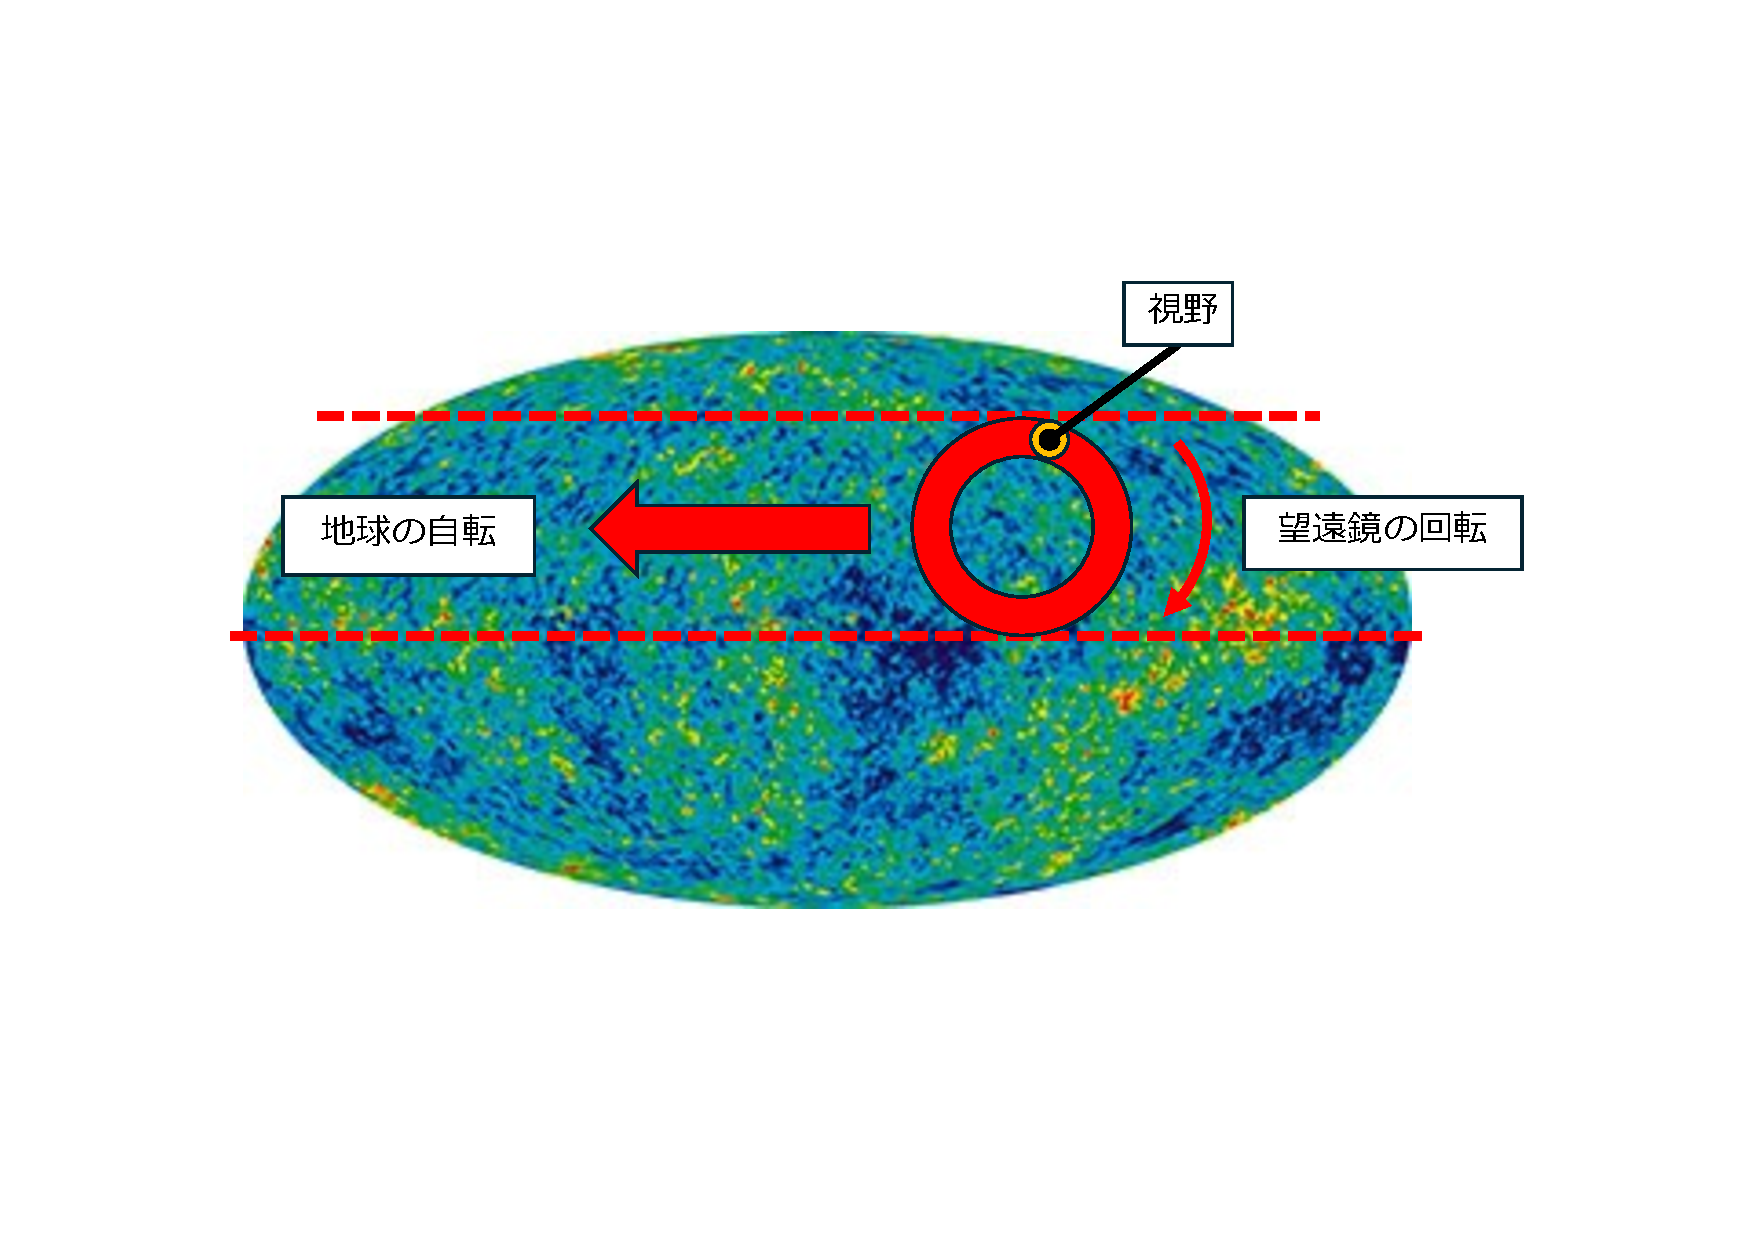
\includegraphics[width=0.8\columnwidth]{3_GB/figs/scan_strategy.pdf}
  \caption{GroundBIRDのスキャン戦略。GroundBIRDは視野$\pm 11^{\circ}$で観測する。望遠鏡の回転と地球の自転を組み合わせることで1日で全天の約半分をカバーできる。}
  \label{scan_strategy}
\end{figure}

次に、GroundBIRDの内部構造の概略を図\ref{GB_inside}に示す。光学系は放物面の主鏡と双曲面の副鏡から成り、CMBがバッフルから入り、光学系で2回反射させた後に、焦点面検出器ステージに入る。クライオスタット内は真空かつ低温になっており、外側のチャンバー部(300K)、40Kシールド、4Kシールドの3層から構成されている。4Kシールドの冷却にはパルスチューブ冷凍機を使用している。GroundBIRDでは超伝導検出器``MKID(Microwave Kinetic Inductance Detector)''を採用しているため、焦点面の温度は極低温に保つ必要がある。焦点面の冷却にはHeソープション冷凍機を使用し、温度を280mK付近に保持している。

\begin{figure}[htbp]
  \centering
  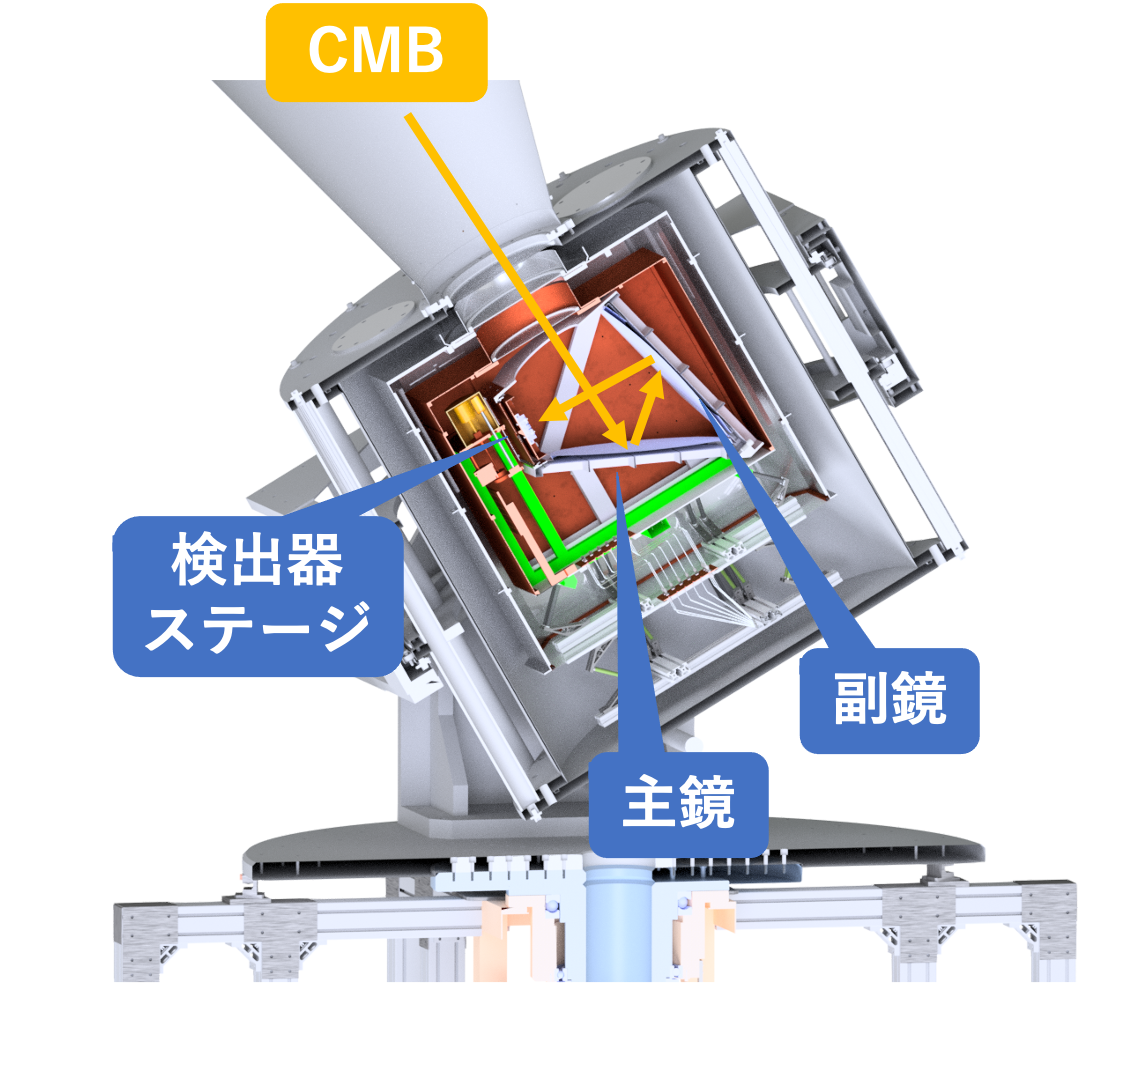
\includegraphics[width=0.6\columnwidth]{3_GB/figs/gb_int.png}
  \caption{GroundBIRD内部の概略図。バッフルを通ってCMBが望遠鏡内に入り、主鏡と副鏡で反射されて検出器ステージに入る。}
  \label{GB_inside}
\end{figure}

\subsection{超伝導検出器MKID}
GroundBIRDでは高速スキャンのもとで角度分解能を失わないようにサンプリングレートを1kHzにしている。そのため、検出器の応答時間が$< \mathcal{O}$(1)msであることが要求される。MKIDの典型的な応答時間は$< \mathcal{O}$(1)msであり\cite{MKID_res}、この要求を満たしている。CMB観測実験では他にも検出器として``TES(Transition Edge Sensor)''ボロメータを使うこともあるが、GroundBIRDでは時間応答性の面からMKIDを採用している。

MKIDの動作原理の概要を説明する。MKIDは超伝導共振回路を応用した高感度な光検出器である。入射する光子のエネルギーに応じて変化する回路内のインダクタンスを、数GHzで読み出す。MKIDの電子顕微鏡写真\cite{MKID_pic}と、等価回路を図\ref{mkid_pic}に示す。MKIDは読み出し線、超伝導体からなる共振器回路、アンテナからなっている。アンテナから電磁波が入射すると超伝導共振器の状態が変化し、そのインピーダンスの変化を読み出すことで入射エネルギーを測定する。

具体的には、検出器の温度上昇やエネルギーが$h\nu > 2\Delta$($\Delta$は超伝導ギャップエネルギー)の光子との反応で、超伝導共振器内のクーパー対(結合した電子対)が壊れる。対になっていた電子はエネルギーギャップより上の準位へと押し上げられる(図\ref{cooper})。この過程で生成される電子を準粒子という。$\Delta$と超伝導転移温度($T_{c}$)の関係は$T$=0Kの時に
\begin{equation}
  2\Delta(T=0) = 3.52k_{B}T_{c}
\end{equation}
と表すことができる\cite{bcs}。ここで、$k_{B}$はボルツマン定数である。この式より、MKIDの材質として用いる超伝導体の転移温度と$\Delta$は1対1対応しており、転移温度を適切に設定することでCMBのエネルギー($\sim 160$GHz)でクーパー対を壊すことができる。例えば、アルミニウムであれば転移温度は1.2Kであり、対応する光子の必要エネルギーは90GHzになるため、CMBの検出が可能になる。また、MKIDでは入射信号によって生成される準粒子の数に比例した応答が得られるため、ギャップエネルギーに近いエネルギーのCMBに対して高感度な検出器になる。

準粒子によって共振器内の超伝導状態が変化し、可変インダクタンスの値が変化する。また、1つの読み出し線に複数の共振器が容量性カップリング(Capacitive coupling; Cカップリング)しており、1対の読み出し配線を使って$\mathcal{O}$(1000)個のMKIDを同時に読み出すことができる。

\begin{figure}[h]
  \begin{tabular}{cc}
    %---- 最初の図 ---------------------------
    \begin{minipage}[t]{0.45\hsize}
      \centering
      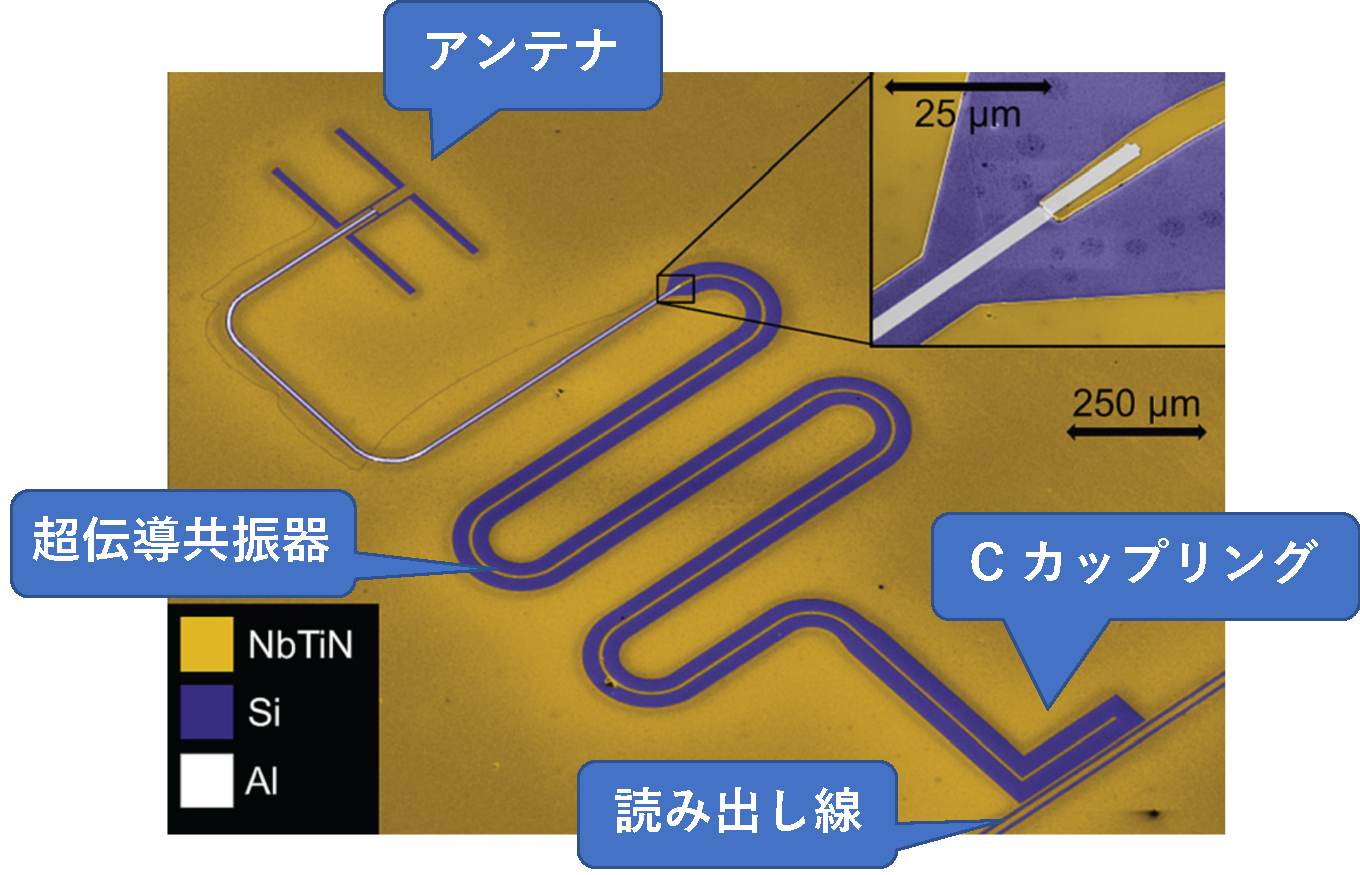
\includegraphics[keepaspectratio, scale=0.3]{3_GB/figs/mkid_pic.pdf}
      \subcaption{MKIDの電子顕微鏡写真\cite{MKID_pic}。読み出し線、超伝導共振器、アンテナからなる。}
    \end{minipage}
    %---- 2番目の図 --------------------------
    \begin{minipage}[t]{0.45\hsize}
      \centering
      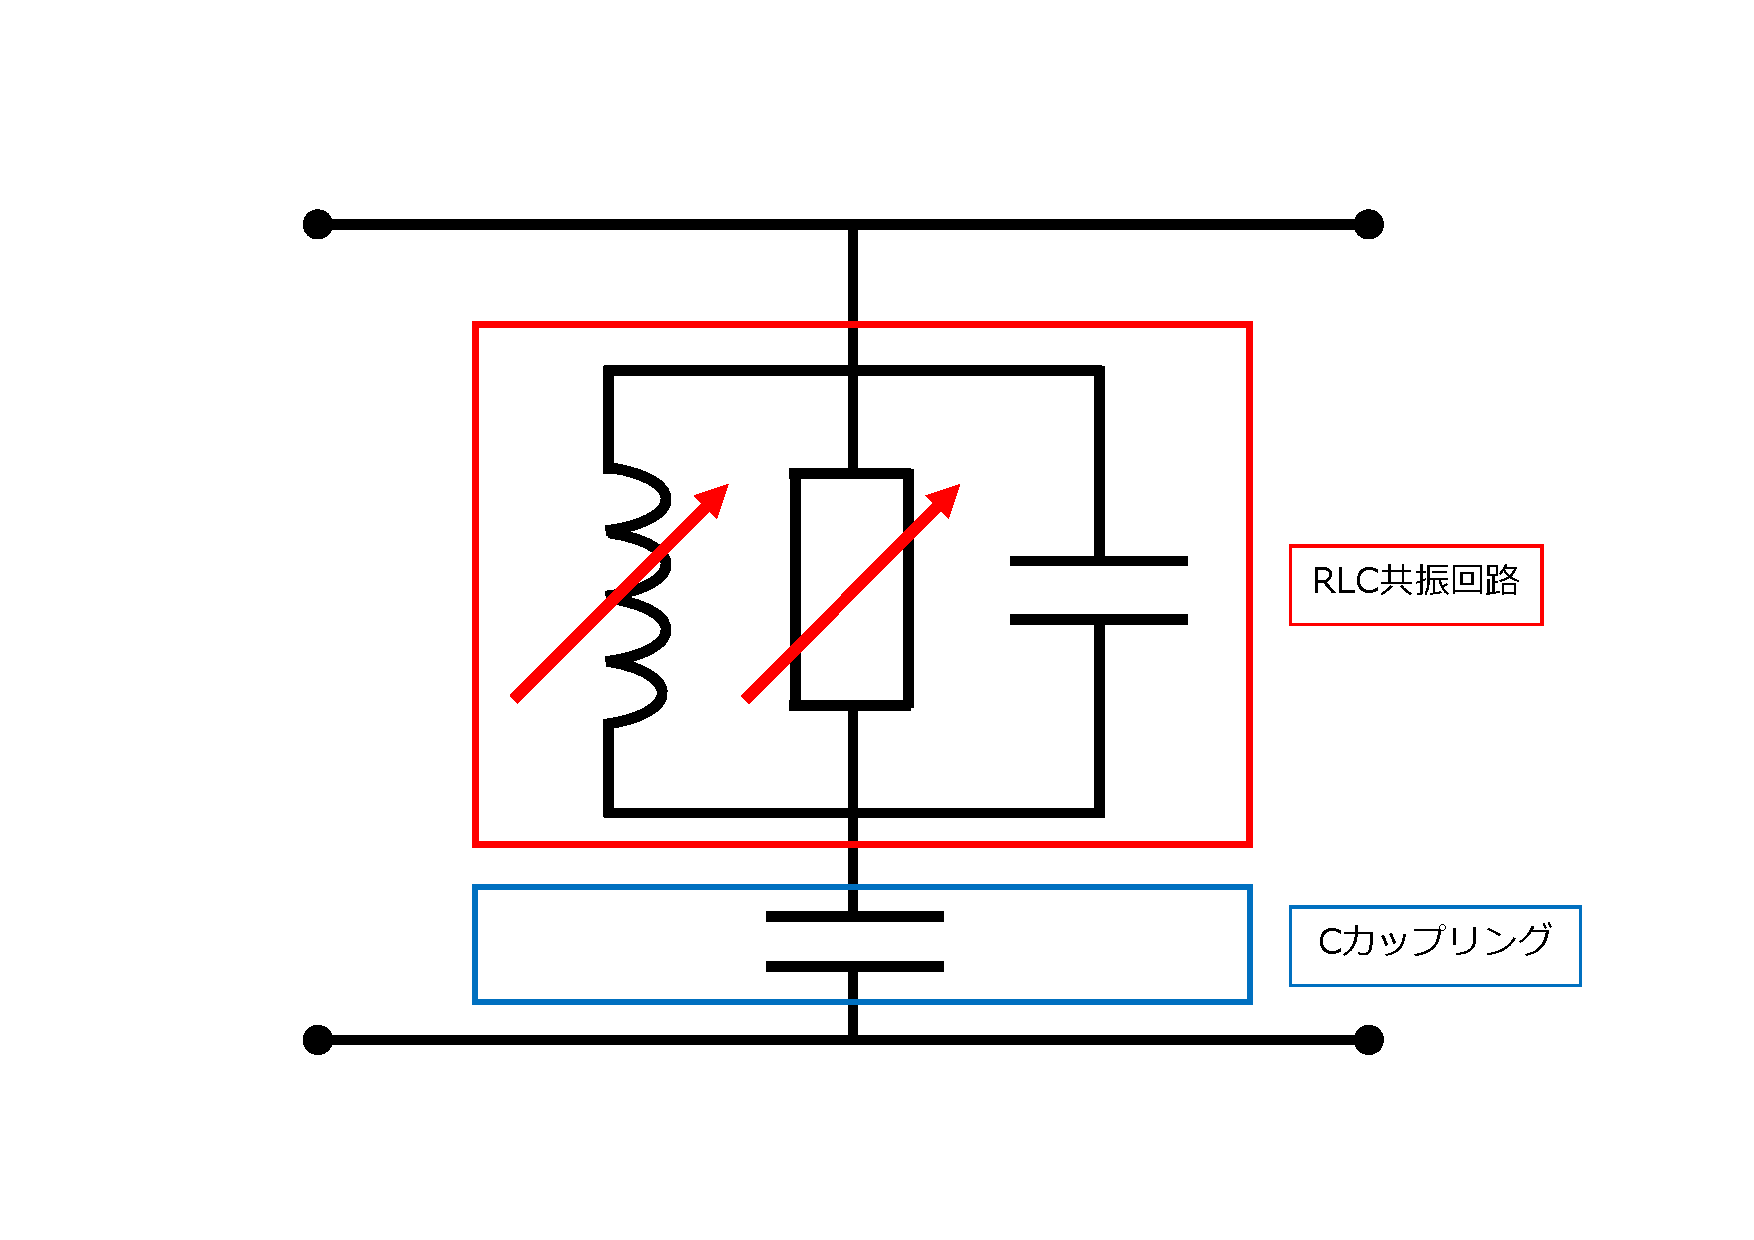
\includegraphics[keepaspectratio, scale=0.3]{3_GB/figs/mkid_circ.pdf}
      \subcaption{MKIDの等価回路。可変インダクタンスと可変抵抗をもつRLC共振回路になっている。}
    \end{minipage}
    %---- 図はここまで ----------------------
  \end{tabular}
  \caption{超伝導検出器MKID}
  \label{mkid_pic}
\end{figure}

\begin{figure}[htbp]
  \centering
  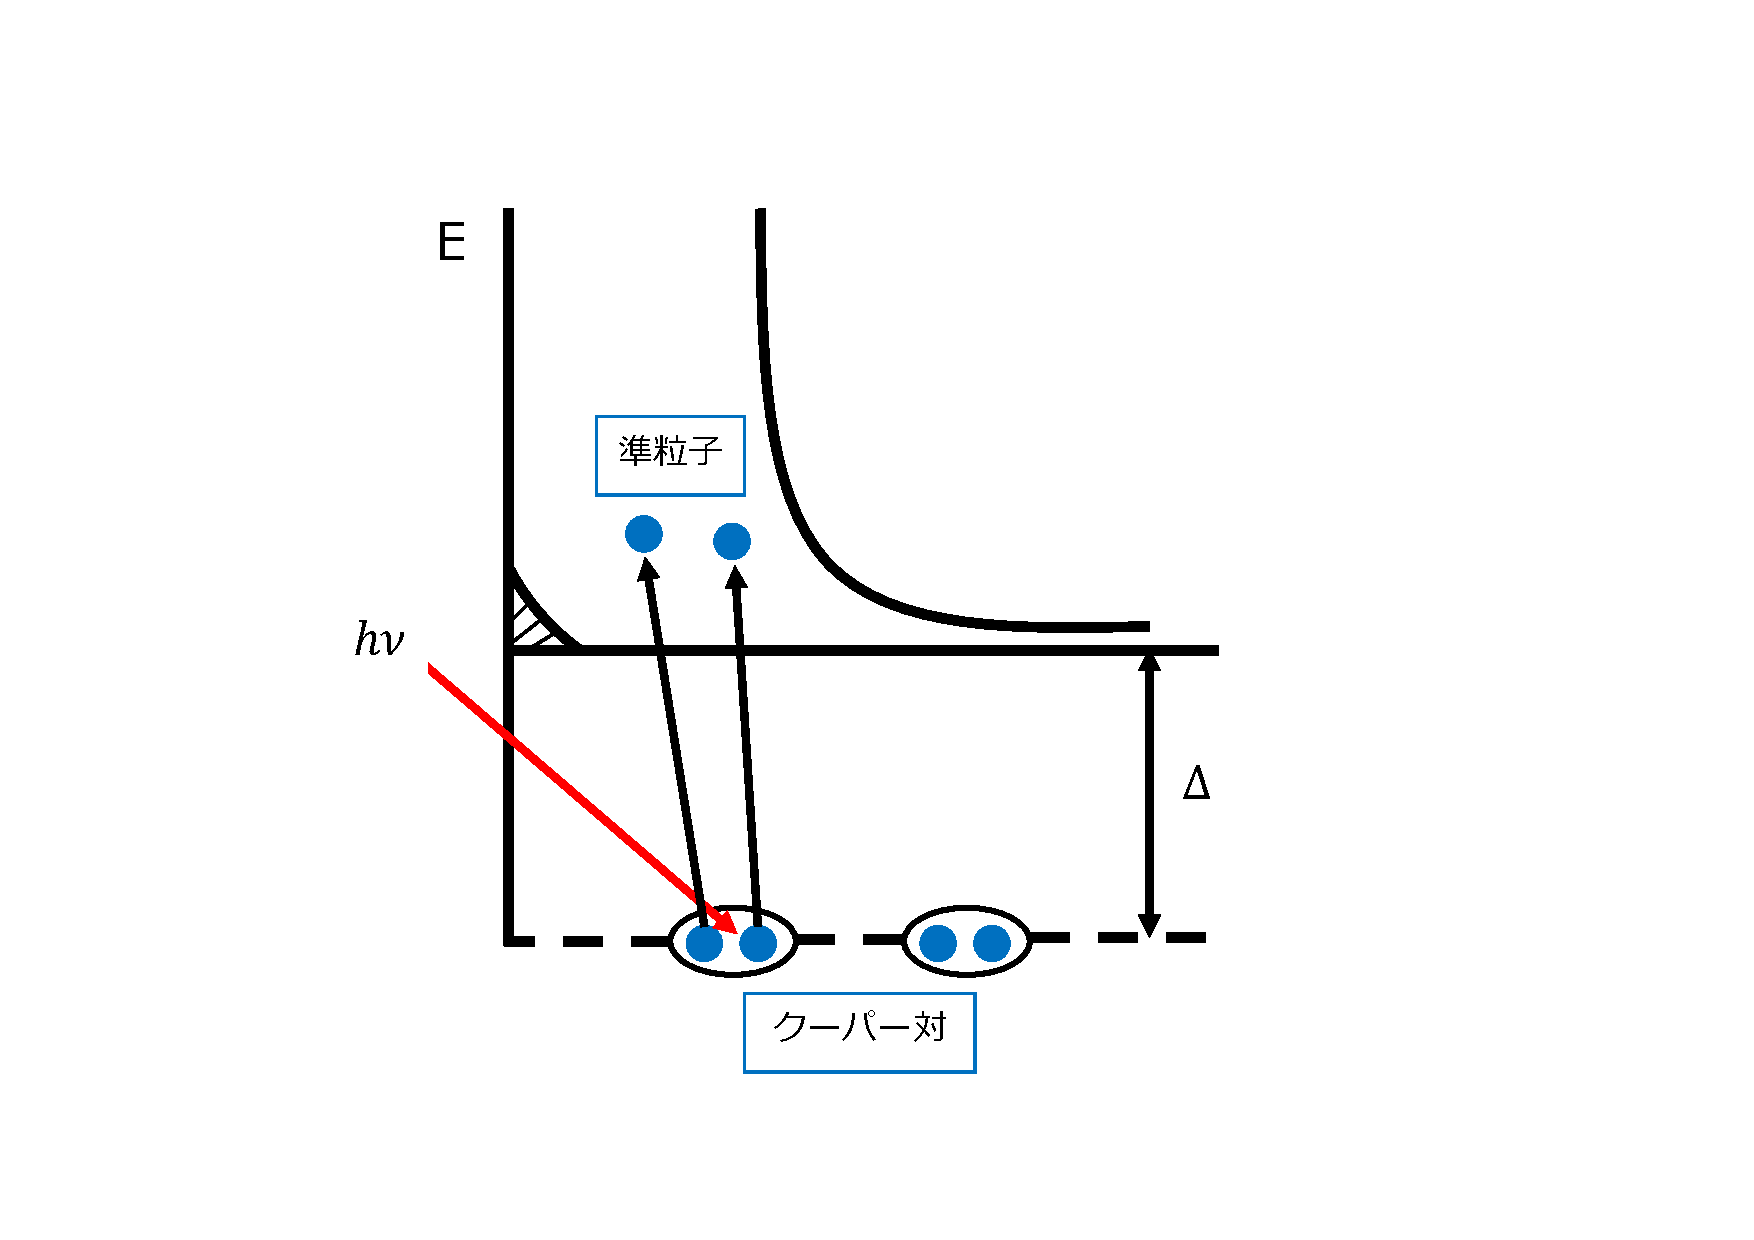
\includegraphics[width=0.6\columnwidth]{3_GB/figs/cooper.pdf}
  \caption{入射光子による準粒子生成の模式図。縦軸は電子のエネルギーを表す。$h\nu > 2\Delta$のエネルギーを持つ光が超伝導共振器に入射すると、クーパー対が壊されてエネルギー準位が押し上げられ、準粒子になる。}
  \label{cooper}
\end{figure}

\subsection{物理ターゲット}
GroundBIRDが探る物理ターゲットは\ref{E_and_tau}で見た光学的厚み$\tau$の地上からの再測定である。光学的厚み$\tau$の測定は今までにWMAPやPlanckといった衛星実験によって測定がされてきた。図\ref{tau_planck}に測定された$\tau$の値の変遷を示す。誤差が小さくなってきており、最新の測定結果ではその誤差は$\sim 10\%$である。しかし、平均値は系統的に下がっている傾向にあり、独立した測定によってこの結果の妥当性を評価する必要がある。そのため、地上実験(例えばCLASS\cite{CLASS}やQUIJOTE\cite{QUIJOTE}など)からの$\tau$の精密測定が始まっている。

\begin{figure}[htbp]
  \centering
  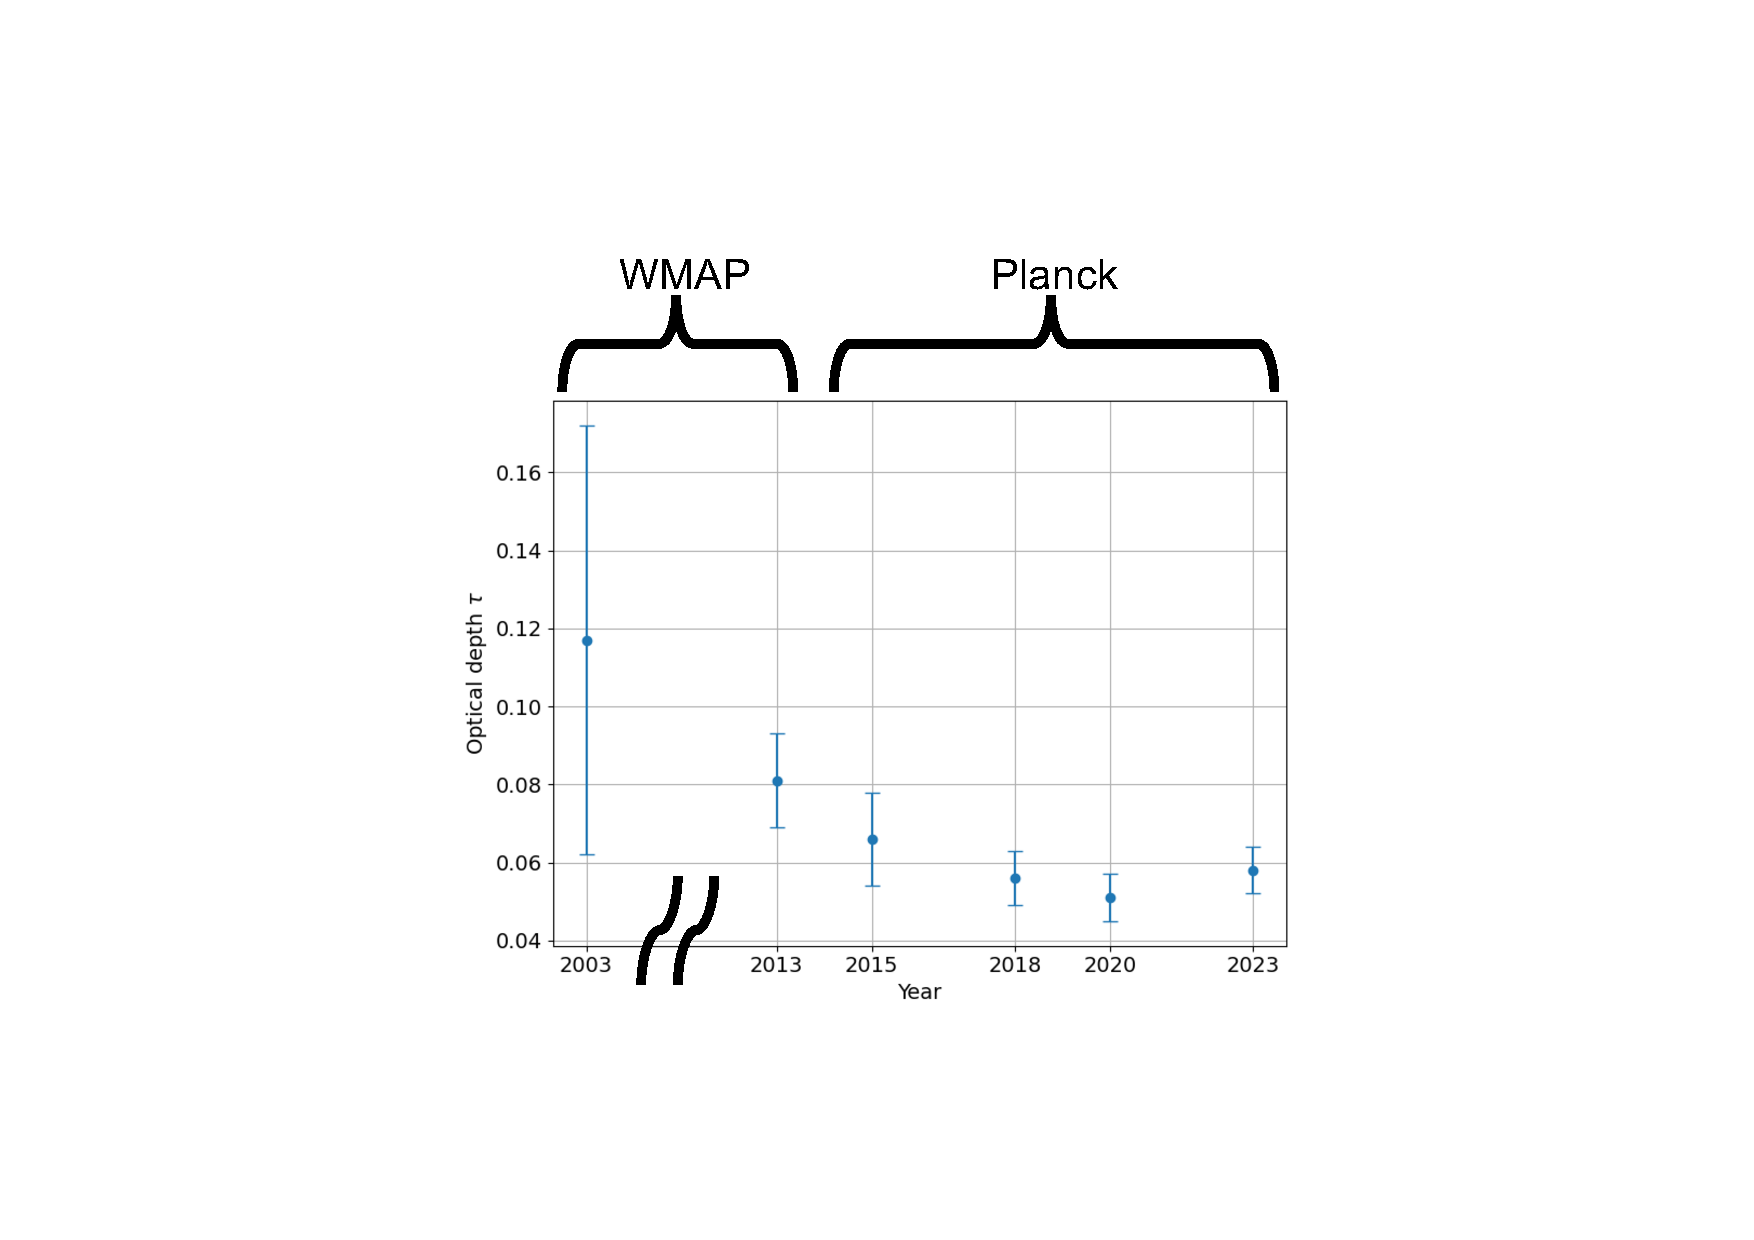
\includegraphics[width=0.8\columnwidth]{3_GB/figs/tau_planck_wmap_cut.pdf}
  \caption{WMAPとPlanckによって測定された光学的厚み$\tau$の値\cite{tau_measure}。最新では誤差は$\sim 10\%$である。}
  \label{tau_planck}
\end{figure}

特にGroundBIRDは独自のスキャン戦略を活かして$\tau$の値に迫ることができる。高速スキャンによって大角度スケール(6 $<\ell<$ 300)のCMB偏光を測定することができる。大角度スケールと$\tau$の関係を図\ref{cl_honda}に示す。偏光Eモードのパワースペクトルは大角度スケール($\geq 10^{\circ}$)で$\tau$に応じて異なる振る舞いをする。GroundBIRDはこの振る舞いを観測することができるため、$\tau$の測定に適している。

\begin{figure}[htbp]
  \centering
  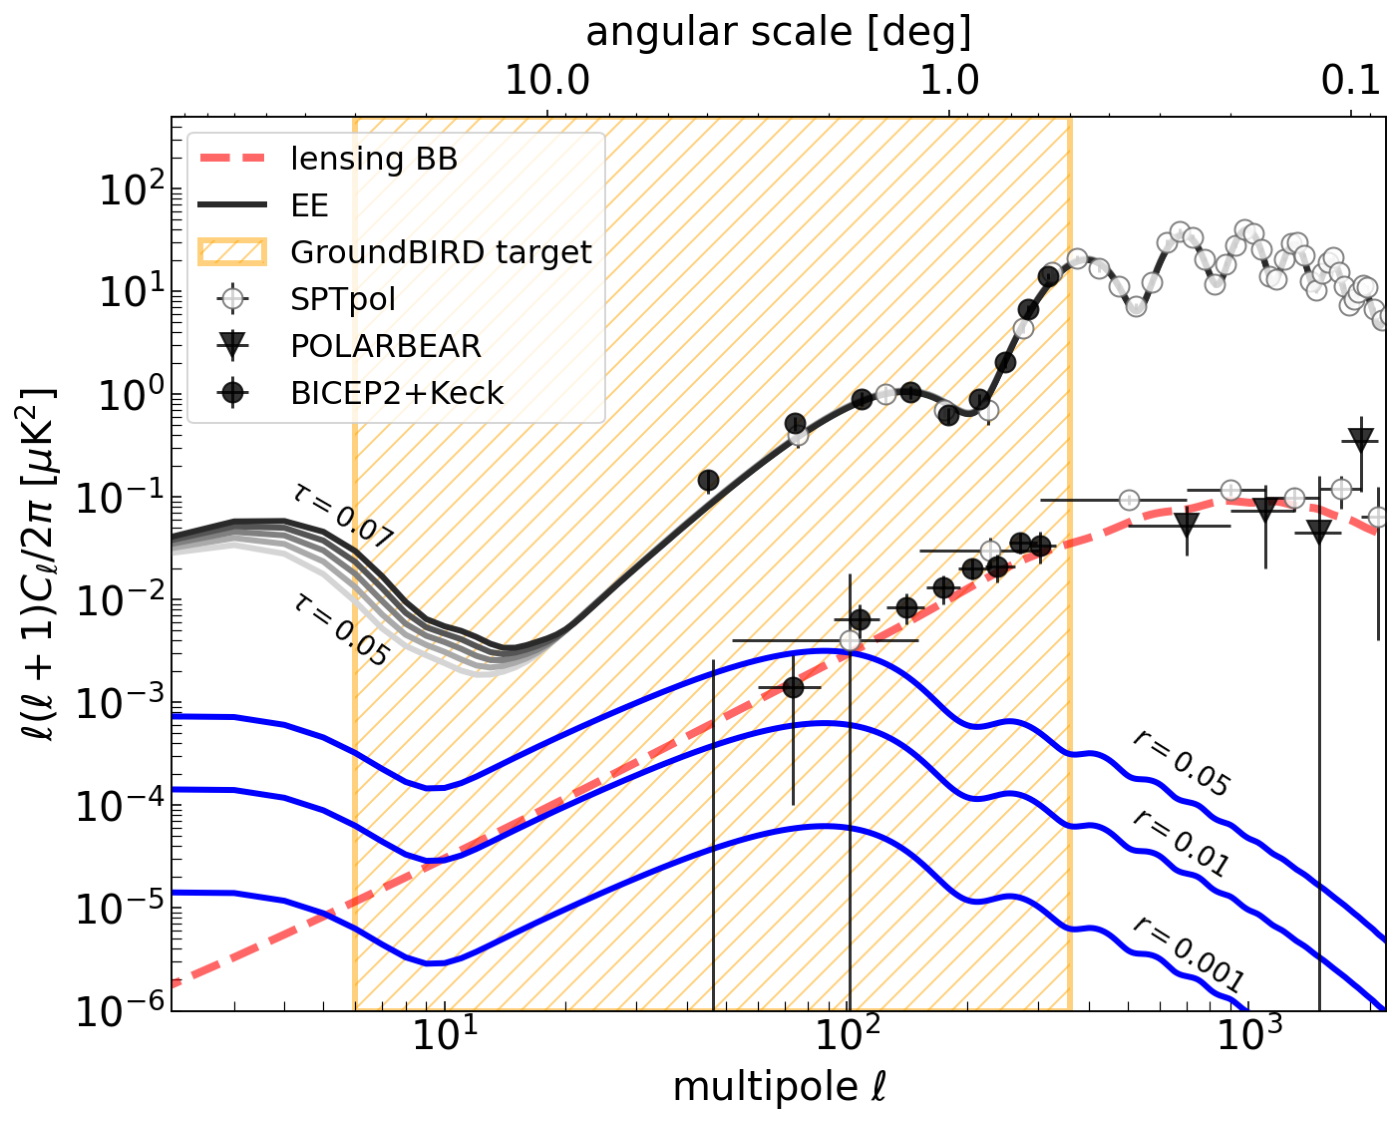
\includegraphics[width=0.8\columnwidth]{3_GB/figs/cl_shonda.pdf}
  \caption{パワースペクトルの過去の観測結果とE,Bモードの理論線、そしてGroundBIRDの観測領域\cite{spie_honda}をオレンジで示す。青実線はテンソル$\cdot$スカラー比を仮定した時の原始重力波由来の偏光Bモード、赤点線は重力レンズ効果由来のBモードを表す。黒実線はEモードであり、大角度スケール($\geq 10^{\circ}$)で$\tau$の値によってスペクトルに違いが生まれる。}
  \label{cl_honda}
\end{figure}

CMB偏光の観測から$\tau$の測定を行うためにはCMBと、銀河などから来るCMBと同周波数帯の放射である``前景放射''とを分離する必要がある。これらの前景放射はそれぞれ異なる周波数依存性を持つ(図\ref{planck_spectrum})。主な前景放射には低周波側で卓越する``シンクロトロン放射''と高周波側で卓越する``ダスト熱放射''があり、CMBにとって大きなノイズとなる。そのため、低周波側$\mathcal{O}$(10)GHzから高周波側$\mathcal{O}$(100)GHzまでの広い帯域での観測を行い前景放射を取り除くことが求められる。\ref{full_array}で述べるが、GroundBIRDはCMBに感度のある145GHzと、ダスト放射に感度がある220GHzの2つの帯域で観測する。一方で、低周波側はQUIJOTE\footnote{QUIJOTE実験はGroundBIRDから20mほどしか離れていない隣に位置する望遠鏡である。}のデータを使うことでカバーする。3年間の観測で、GroundBIRDとQUIJOTEの共同解析によって$\tau$を誤差$\sigma_{\tau}\sim$ 0.01で測定することを目指す\cite{joint_ana}。

\begin{figure}[htbp]
  \centering
  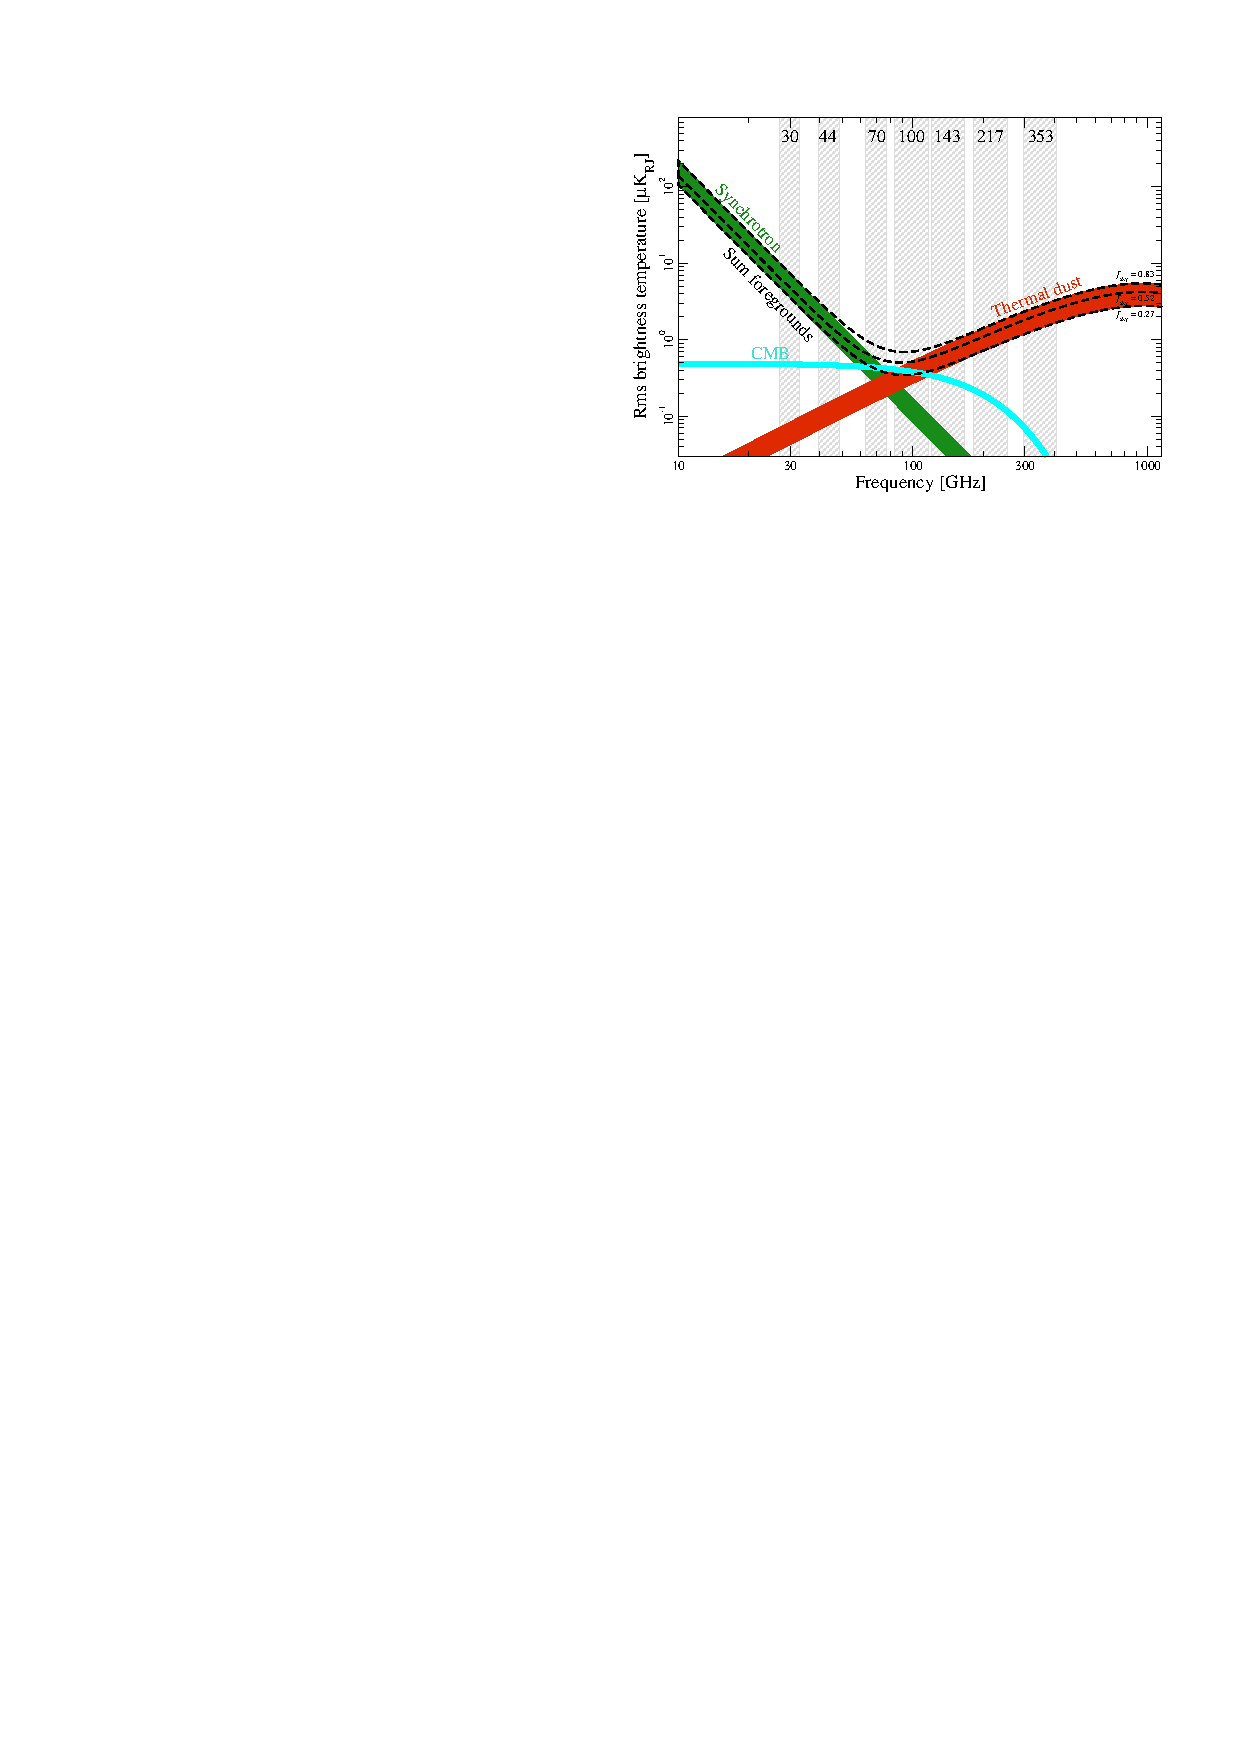
\includegraphics[width=0.8\columnwidth]{3_GB/figs/planck_spectrum.pdf}
  \caption{CMBと前景放射の偏光強度を周波数の関数として表した図。Planck\cite{planck_cmb}を参照。それぞれの前景放射は異なる周波数依存性を持ち、CMBとこれらを分離するためには広い帯域での観測が必要になる。}
  \label{planck_spectrum}
\end{figure}

\section{現在の観測状況}

\subsection{検出器のフルアレイインストール}
\label{full_array}
GroundBIRDの現在の状況について説明する。2022年1月から2022年5月まではプロトタイプ検出器を用いたコミッショニング観測が行われた。コミッショニングデータを用いて望遠鏡の視線方向の較正\cite{sueno_paper}や、偏光角較正、ノイズ特性の理解\cite{sueno_doctor}などがされてきた。並行して、2023年5月に全焦点面検出器のインストールが完了し、本格的な物理観測がスタートした。

インストールした焦点面検出器を図\ref{full_array_mkid}に示す。23個のMKIDが1つのアレイに搭載されており、145GHzが6アレイと220GHzが1アレイの全7アレイからなる。中央に220GHzアレイがあり、その周りを145GHzアレイが囲むように並んでいる。アレイごとに読み出しを行う。アレイ内でのMKIDの配置は図\ref{mkid_design}にようになっている。各MKIDは片偏波アンテナを持つため、1方向の偏光方向に感度がある。また、偏光方向は$45^{\circ}$ずつで4方向あり、異なる方向に感度のあるMKID同士で交互に配置されている。これにより、第\ref{chapter4}章で述べるような検出器間で差分を取る解析によって偏光測定をすることができる。

\begin{figure}[htbp]
  \begin{tabular}{cc}
    %---- 最初の図 ---------------------------
    \begin{minipage}[t]{0.49\hsize}
      \centering
      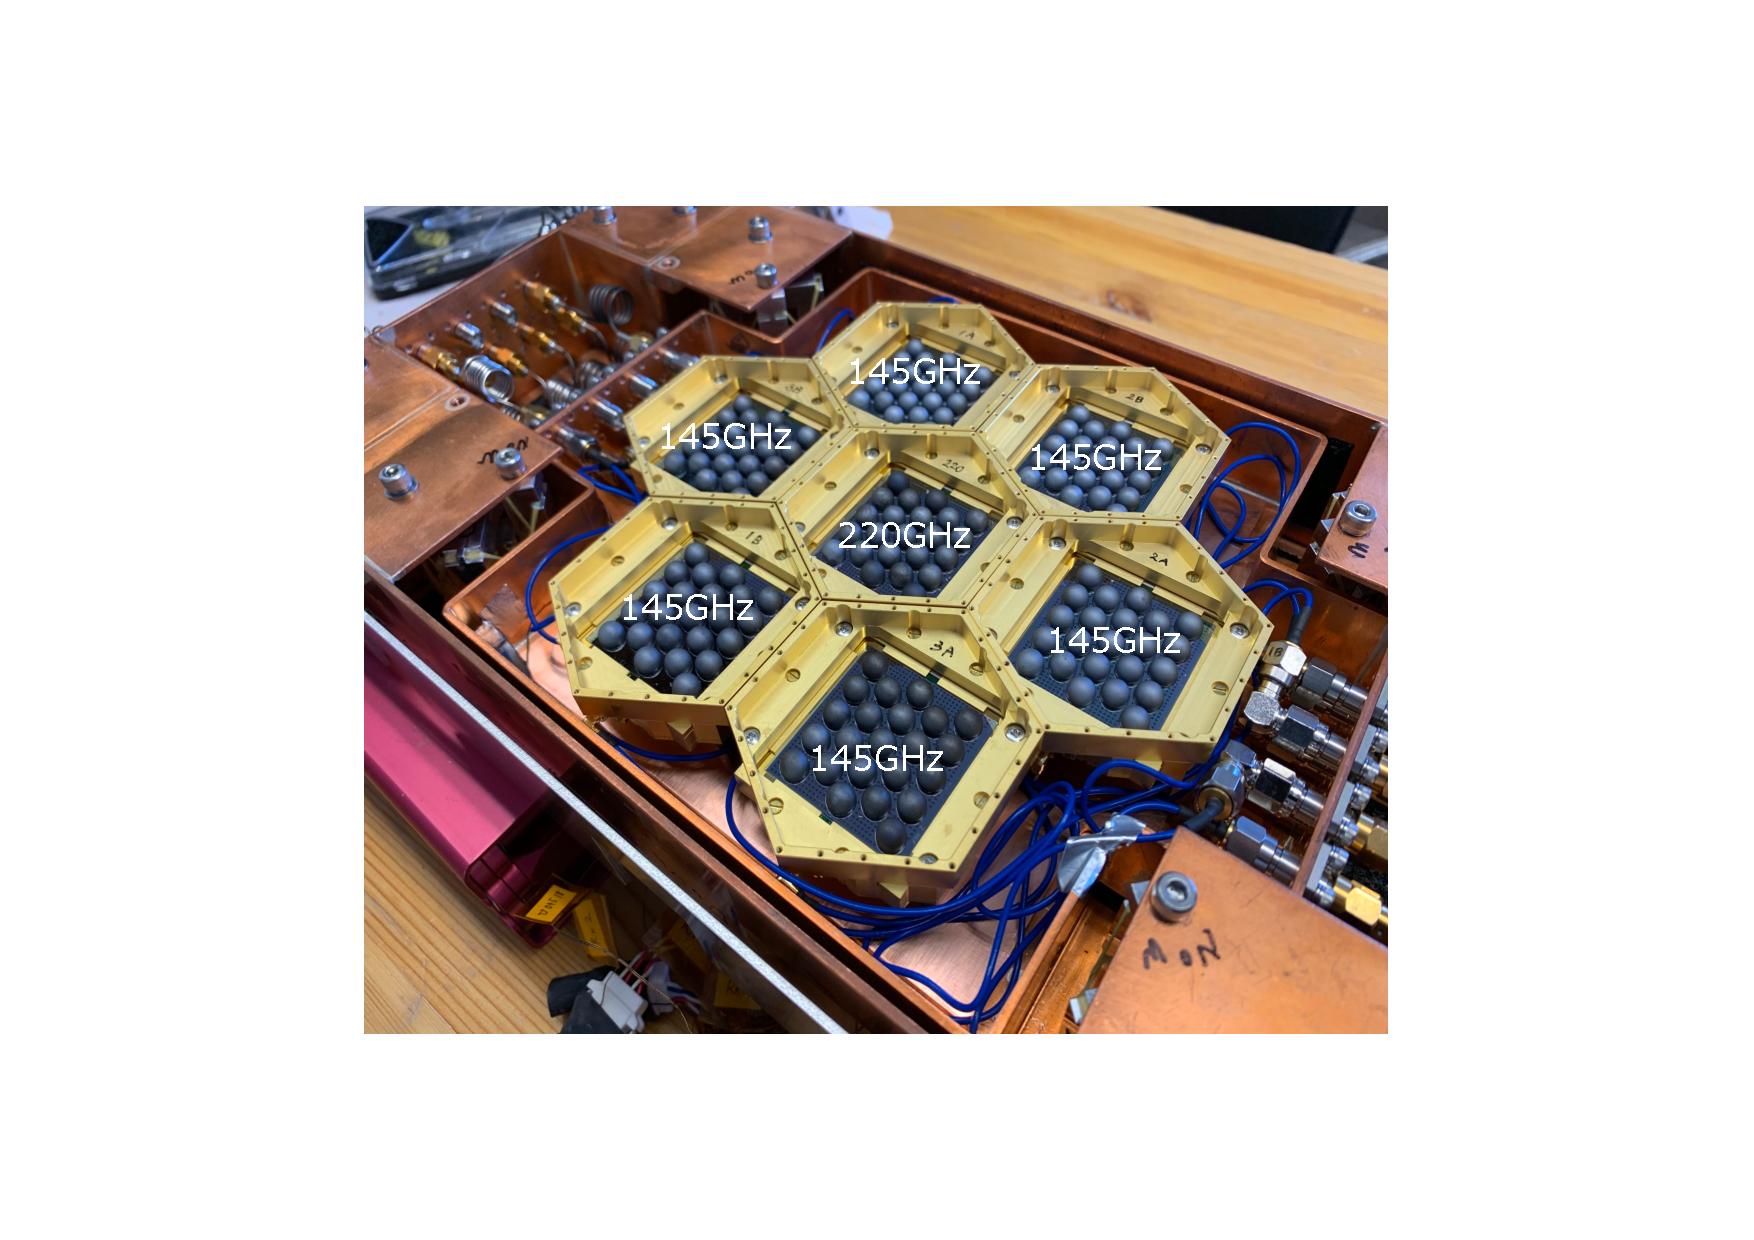
\includegraphics[keepaspectratio, scale=0.37]{3_GB/figs/full_array.pdf}
      \subcaption{焦点面検出器の全体写真。}
    \end{minipage}
    %---- 2番目の図 --------------------------
    \begin{minipage}[t]{0.49\hsize}
      \centering
      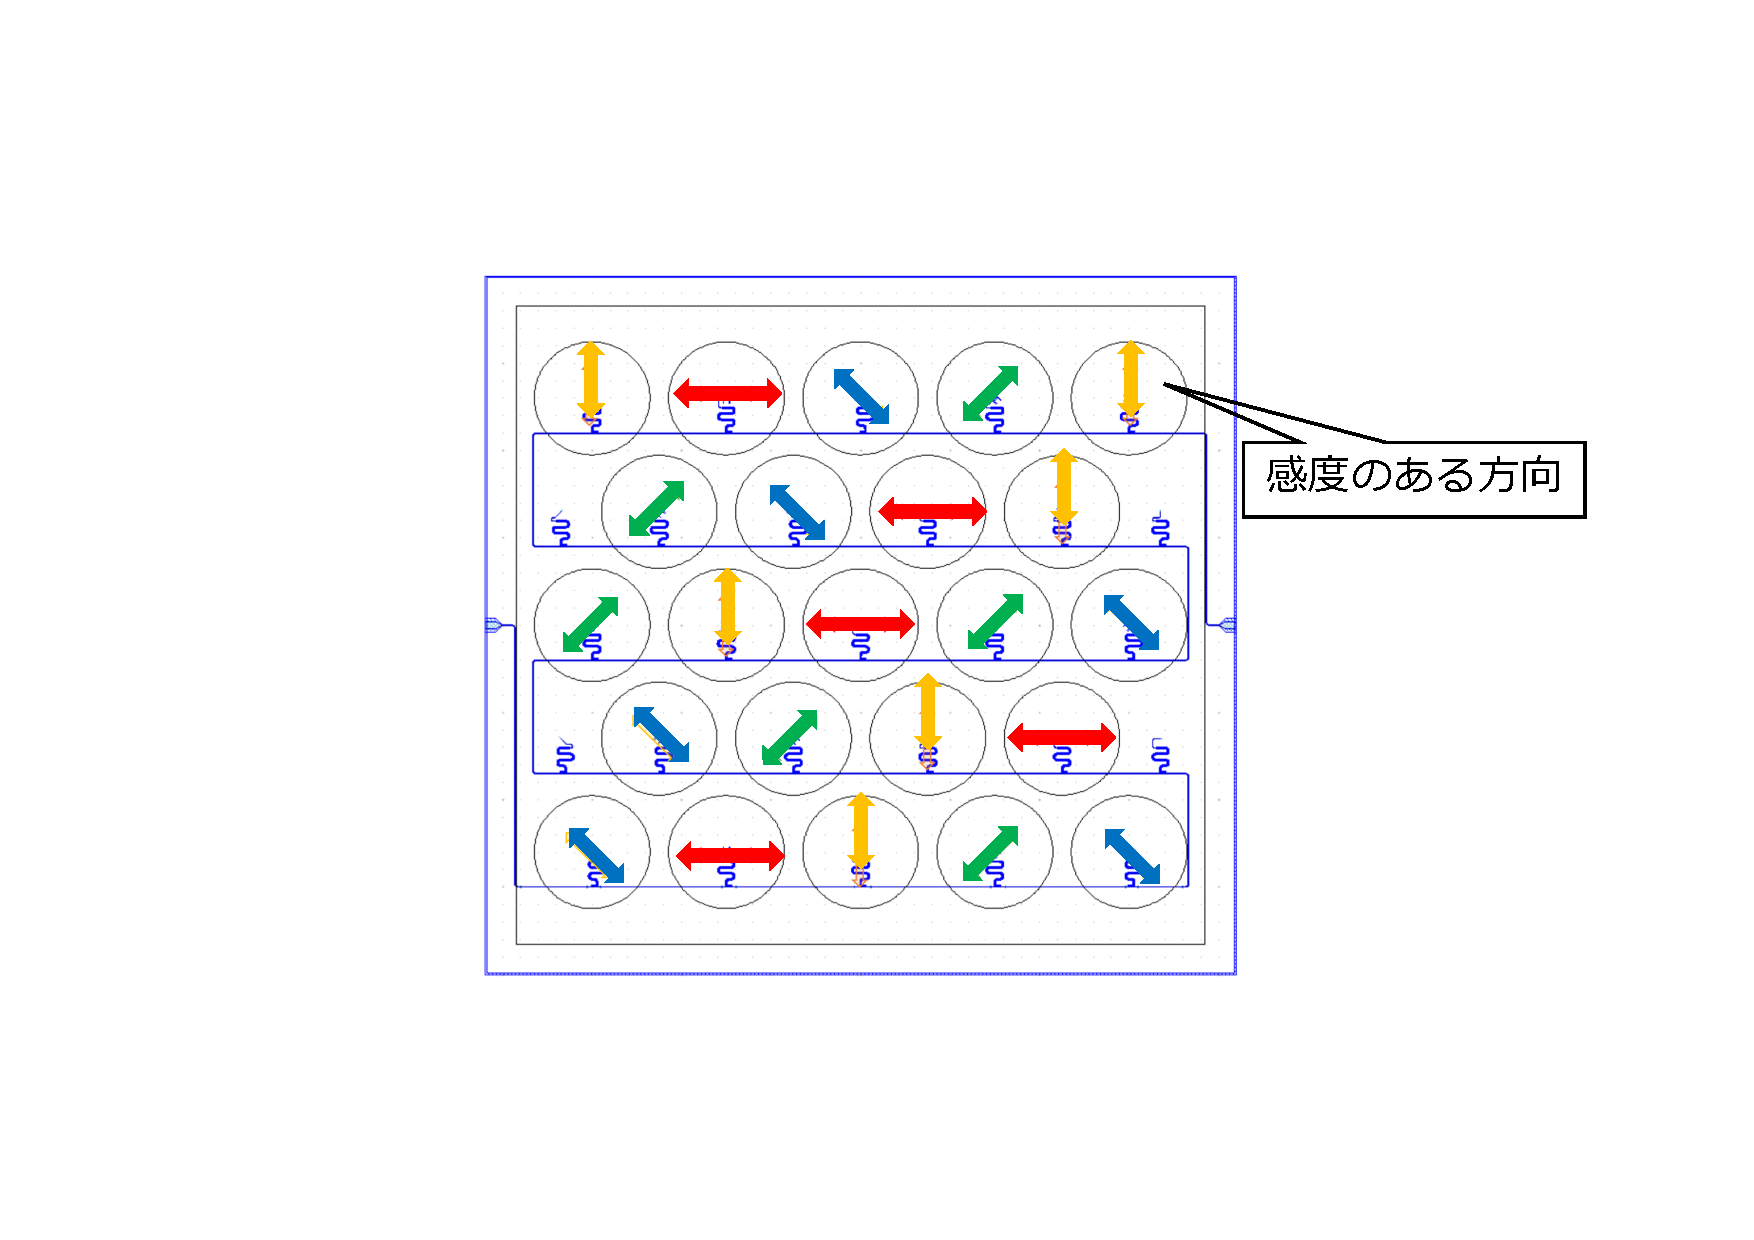
\includegraphics[keepaspectratio, scale=0.43]{3_GB/figs/mkid_design.pdf}
      \subcaption{アレイ内のMKIDが感度を持つ偏光方向。}
      \label{mkid_design}
    \end{minipage}
    %---- 図はここまで ----------------------
  \end{tabular}
  \caption{フルアレイの焦点面検出器MKID}
  \label{full_array_mkid}
\end{figure}

最後に145GHz, 220GHzのそれぞれの検出器と望遠鏡ビームの特性を表\ref{mkid_table}に示す。

\begin{table}[htbp]
  \centering
  \caption{145GHz、220GHzにおける検出器とビームの特性\cite{choi_doctor}}
  \vspace{3mm}
  \begin{tabular}{ccc} \hline
    & 145GHz & 220GHz \\ \hline
    MKID数 & 6アレイ(138ピクセル) & 1アレイ(23ピクセル)\\
    ビーム幅(FWHM) & $0.60^{\circ}(36')$ & $0.42^{\circ}(25')$\\
    ビーム楕円率 & $ < 1\% $ & $ < 2\% $\\ \hline
  \end{tabular}
  \label{mkid_table}
\end{table}

\subsection{リモート観測システム}
焦点面検出器のフルアレイインストール後、本格的な観測が始まっているが、基本的に全ての操作(ドームの開閉、望遠鏡の回転など)をリモートから行なっている。観測の手順は以下のようにして行う。
\begin{enumerate}
  \item 天候等が観測に十分適しているか確認
  \item 問題がなければドームを開き、望遠鏡の回転を開始
  \item 検出器のデータ取得を開始し、観測状況をモニター
\end{enumerate}
望遠鏡をダストや雨、直射日光から守るために観測時間以外はドームを閉めている。観測開始前には天候状況(PWV、湿度、風速等)を確認し、観測するか否かを判断する。また、日光が望遠鏡の視野に入る日中や、冷却に使用するHeのメンテナンス時間以外は基本的に観測を継続する。そのため、観測シフトを日本時間と現地時間で分けることで1日を通して観測を続けている。また、Slackアプリケーションを導入し、アプリ内で対話的に観測状況を把握できるようになっている(図\ref{samesan})。

\begin{figure}[htbp]
  \centering
  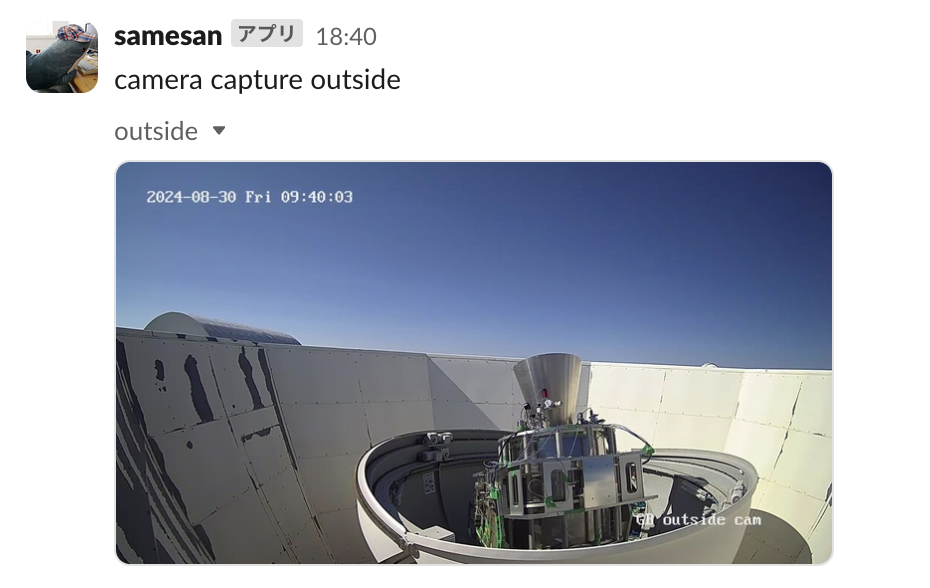
\includegraphics[width=0.6\columnwidth]{3_GB/figs/webcam.png}
  \caption{Slackアプリケーションを用いたモニター。Webカメラの映像から観測状況を確認できる。他にも観測中の検出器データのチェックや、サウンドモニターによる異音検知などが可能。}
  \label{samesan}
\end{figure}

%\section{本論文の構成}
%ここまで第\ref{chapter1}章でCMBに関わる理論的な背景、第\ref{chapter2}章でGroundBIRD実験の概要を説明した。以降は第\ref{chapter3}章と第\ref{chapter4}章の2部構成になっており、第\ref{chapter3}章でGroundBIRDの角度データ取得システムの改善について、第\ref{chapter4}章で焦点面検出器のアライメント較正とその結果について述べる。第\ref{chapter5}章で今後の展望を述べ、第\ref{chapter6}章でまとめを述べる。
